\textbf{\textit{``capturing and recording information on adverse events, and analysing them in the right way is an essential step to reducing risk to patients...''}}

Building a safer NHS for patients, Department of Health Report 2001 




\chapter{Introduction}

\section{Overview}
I am a medical doctor and an amateur software developer who has recently returned to clinical work from a secondment with the \gls{NPSA}. I have chosen to approach the question posed by the title of this thesis primarily from within the organizational context of the \gls{NPSA}. To keep the project manageable I analyse only the specific subset of patient safety incidents that relate to computer problems and limit the data mining approaches considered.

The thesis is set out in four main parts, in part \ref{Background} I characterize the problem I will address and describe aspects of the \gls{NPSA}'s work, patient safety, and machine learning. In part \ref{Method} I describe and justify the data mining methods used. In part \ref{Results} I document the results I have obtained and explain their significance. In part \ref{Conclusion} I discuss my results in the context of the question posed by the thesis and set out my conclusions.

\section{Problem statement}
Over one million incidents are reported to the \gls{NRLS} per year, many more than would be humanly possible for the staff to manually review. Therefore in NRLS practice, routine analysis, and learning, is limited in the main to incidents which are reported to have caused serious harm or death. A consequence of this is that there exists potentially significant unknown patterns, and learning, in the large number of incidents that it is not practicable to review centrally. 

It is not known whether data mining can facilitate learning from patient safety incidents. Answering this is a hard problem. In order to proceed I will limit this thesis to consideration of the specific subset of patient safety incidents concerning computer problems. I will also limit the datamining approaches used to testing data exploration and auditing tools, the Lingo clustering algorithm, and Naive Bayes (NB) and Stochastic Gradient Descent (SGD) severity classifiers. Specifically, I will consider the following two questions in relation to patient safety incidents concerning computer problems:

\begin{enumerate}
 \item Can free text incident descriptions be analysed in an automated fashion to generate meaningful groupings (clusters)?
 \item Can the severity of harm arising from a patient safety incident be predicted using free text incident descriptions (using a classifier)?
\end{enumerate}

In current practice similar incidents are grouped together in order to find common modifiable causes and inform prevention strategies. Taxonomy construction and application to incident data facilitates human understanding of the data. However, matching and taxonomy construction is time consuming and necessarily limited in scope and granularity by the preconceived categories selected to be in the taxonomy. In virtue of being a machine process unsupervised machine learning in the form of clustering is less time consuming and can be more dynamic. Further, it may provide new insights into the the incident data and suggest new categories. 

Classifying the severity of incidents occurring is important to prioritize and target remedial efforts. Incident severity is included in the initial incident report but misclassification is a known problem.\cite{Niland2012}\cite{Ong2012} An automated classifier may help to flag incidents that are misclassified and assist in central review of incident severity classification. \label{missclassifcation_problem}

\section{The NPSA}
The \gls{NPSA} was formed in 2001 following the publication of two landmark reports by the then Chief Medical Officer, Professor Sir Liam Donaldson. An organization with a memory\cite{CMO2000} and Building a safer NHS\cite{CMO2001} set out the need for greater organizational learning from safety incidents to make the NHS safer for patients. \cite{Stephenson2005}

\subsection{Patient safety and incident reporting}
Recognising that a `blame and punish' culture can inhibit reporting of safety incidents the Department of Health and the \gls{NPSA} placed emphasis on the role of systems, rather than individuals acting alone, in safety incidents. Drawing inspiration from risk management in aviation, where a safety culture and incident reporting are the norm, NHS employees are now actively encouraged to report safety incidents.

\paragraph{What is a patient safety incident?}
A \gls{patient safety incident}, also called an adverse incident, occurs whenever something unexpected happens as part of medical care that harms, or nearly harms, a patient.

\paragraph{How do health care professionals report safety incidents?}
Healthcare professionals report safety incidents to the \gls{NRLS} using a standardized incident reporting form. This form, called an IR1 form, is usually paper based but may also be electronic.\cite{ReportAnIncident} The form serves as a means for the healthcare professional to inform his or her institution when an incident has occurred.

\paragraph{What is contained on an incident report form?}
\label{incidentreport}
Incident reports record the following information:
\begin{enumerate}
 \item The facts of the incident (including a free text description)
 \item The perception of possible consequences (the potential or actual harm)
 \item The perception of how the incident came to arise (the cause or causative factors)
\end{enumerate}

\paragraph{What happens to incident report forms?}
Incident report forms are reviewed, and investigated further if necessary, by the local clinical governance team. All incident forms are then submitted electronically to the \gls{NRLS} for national level analysis.

\subsection{The National Reporting and Learning Service (NRLS)}
The \gls{NRLS} is the division of the \gls{NPSA} concerned with the analysis of reports of patient safety incidents and safety information from other sources. On the basis of this analysis the NRLS develops and issues safety alerts to NHS organizations such as acute hospital trusts.

Safety alerts aim to reduce preventable harm to patients by raising awareness of threats to patient safety and recommending steps to reduce the risk of these threats. Alerts are typically issued is response to the identification of specific under-recognized threats to patient safety. These are threats identified through the incident reporting system that have proven to cause death or serious harm, are likely to recur, and are at least theoretically amenable to preventative measures or changes of practice. 

For example, when the NPSA became aware that there were several patient deaths a year in the United Kingdom due to the accidental administration of potassium chloride solutions, it established that the main causes of accidental administration resulted from the drug being stored in the same place, and having similar packaging to, other commonly used drugs such as frusemide and normal saline. Hence, the incident was potentially preventable by changing how potassium chloride is stored and packaged. The NPSA then issued a safety alert regarding potassium chloride solutions which included specific recommendations regarding the storage, packaging, and handling of potassium chloride solutions and the rates of accidental potassium chloride administration fell.

A key premise of the NPSA's work is that incident reporting, the NRLS, and alerts can improve patient safety by allowing learning from incidents and near misses\cite{Smith2009}. This model of incident reporting and learning has been successful in other high risk industries such as aviation where with time the number of incidents has increased but the total number of incidents causing death or serious harm has fallen.

Over one million incidents are reported to the NRLS per year, many more than would be humanly possible for the staff to review. Therefore routine analysis, and learning, is limited in the main to incidents which are reported to have caused serious harm or death. A consequence of this is that there are potentially additional, as yet undiscovered, patterns and learning in the large number of incidents that are not analysed centrally. 

\section{Data mining} %consider rewrite in terms of machine learning from scikit and add stuff from macky
\subsection{What is data mining?}
\gls{DM} is the analysis of (often large) observational data sets to find unexpected relationships and to summarize the data in novel ways that are both understandable and useful to the data owner.\cite{Hand2001} In order to achieve understandable and useful insights, DM requires input from experts with domain knowledge.

Historically, data mining has been conceived of as a step in the \gls{Knowledge Discovery in Databases} (KDD) process.\cite{Fayyad1996} That is the discovery of knowledge from a database involving the selection of data, preprocessing, transforming, mining to extract patterns and relationships, and then interpreting and assessing the discovered structure.

More recently, the term \gls{DM} has been used to refer to the KDD process itself and I use the term this way. Incidentally, use of the term \gls{Data Science} has recently emerged to refer to this process where the data being manipulated is large, gigabytes or more at the time of writing (\gls{Big Data}).

\gls{DM} draws heavily on statistical techniques from machine learning which are about building programs or models with tunable parameters that adjust automatically and improve their behaviour by adapting to previously seen data.\cite{Vanderplas2012}

\gls{DM} is non-linear, iterative, and intimately related to the selection of data, data preprocessing, and data transformation. Therefore, in this thesis I use \gls{DM} to refer to the whole process, from obtaining data to arriving at valuable interpretations of it. I also use the term to refer to both descriptive and predictive analytic methods.



\subsection{Techniques used in data mining} %?add picture from scikit

\gls{DM} may be broken up into three stages that mirror the extraction, transformation, and load (ETL) pattern (see section ~\ref{fig:dataminingoverview} also):

\begin{enumerate}
 \item Data acquisition (extraction)
 \item Data processing and analysis (transformation)
 \item Evaluation, interpretation, and tuning (loading)
\end{enumerate}

\subsubsection{Data cleaning and audit}
The first step of data processing in DM is typically data cleaning and audit. This includes removing duplicates and reconciling spelling variants and acronyms as well as auditing the data. Typical audit tasks would include identifying the types of data field present and how often they are completed within the data sample. 

\subsubsection{Exploring data}
Analysis of a large textual data sample may begin with inpection of a manageable subsample or a search of the data for topics of interest which might be present.

Techniques are discussed in more depth in chapter~\ref{chap:dataanalysis}. At root, quantitative analysis techniques used in data mining are statistical in nature. They may be used either to describe, and gain new insight into, existing data, or, to build models from existing data to make predictions for new data. The advent of widely accessible computing power and data has led to a significant growth in the number of people carrying out these types of data analysis. In turn, the number of tools available has increased proportionally and applications outside of traditional business analysis and science have become widespread.

The two specific machine learning techniques I will consider in more depth in this thesis are:
\begin{itemize}
 \item Clustering
 \item Classification
\end{itemize}

\subsubsection{Clustering}
\label{clusteringintro}
Clustering is an unsupervised machine learning technique in which similar samples in a dataset are automatically placed together into distinct groups, or clusters, by an algorithm.

\begin{figure}[htp]
\centering
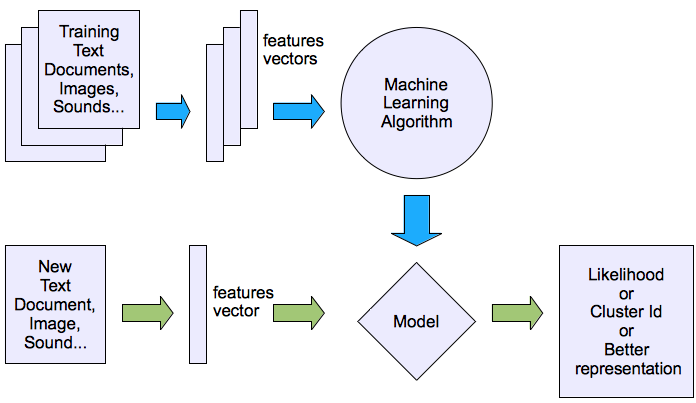
\includegraphics[width=15cm,height=10cm]{figs/unsupervised.png}
\caption{Unsupervised learning overview. An unlabelled data set is used to build a model that best summarizes regularities found in the data. The two main techniques in unsupervised machine learning are dimensionality reduction and clustering.\cite{Pedregosa2011}}\label{fig:unsupervisedlearningoverview}
\end{figure}

Some common applications of clustering algorithm include\cite{Pedregosa2011}:

\begin{itemize}
 \item Building customer profiles for market analysis
 \item Grouping related web news (e.g. Google News) and websearch results
 \item Grouping related stock quotes for investment portfolio management
 \item Can be used as a preprocessing step for recommender systems
 \item Can be used to build a code book of prototype samples for unsupervised feature extraction for supervised learning algorithms
\end{itemize}

The other main unsupervised learning technique, which is not considered in depth here, is dimensionality reduction. In dimensionality reduction the task is to derive a new set of artificial features that is smaller than the original feature set while retaining most of the variance of the original data. This can be useful for allowing visualisation of high dimensional datasets and as a preprocessing step in computationally intensive supervised learning methods.

\subsubsection{Classification}
\label{classificationintro}
In classification a supervised learning algorithm is used to build a predictive model (a classifier) from a labelled dataset. The classifier operates on new unlabelled data to predict the label. For example, a classifier may be built to label new emails as spam, normal or priority mail using a collection of old emails which have been manually labelled by a human. Common applications of classifiers include:

\begin{table}[htbp]\centering
\begin{tabular}{l p{5cm}}
\toprule
\textbf{Task} & \textbf{Predicted outcomes} \\
& \textbf{(labels)} \\
\midrule
E-mail classification & Spam, normal, priority mail \\
Language identification in text documents & en, es, de, fr, ja, zh, ar, ru... \\
News articles categorization & Business, technology, sport... \\
Sentiment analysis in customer feedback & Negative, neutral, positive \\
Face verification in pictures & Same / different person \\
Speaker verification in voice recording & Same / different person  \\
\bottomrule
\end{tabular}
\label{tab:classifier_applications}
\caption{Example applications of classifiers.\cite{Pedregosa2011}}
\end{table}

\begin{figure}[htp]
\centering
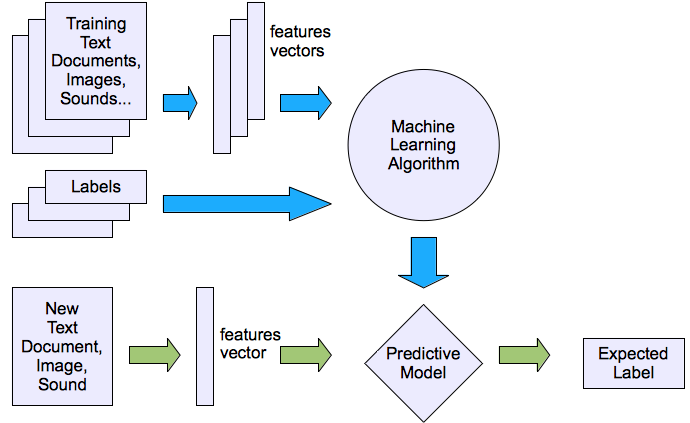
\includegraphics[width=15cm,height=10cm]{figs/supervised.png}
\caption{Supervised learning overview. A labelled data set is used to train a predictive model that can then predict labels for new unlabelled data. When the labels are categorical variables the task is called classification. When the labels are continuous variables the task is called regression.\cite{Pedregosa2011}}\label{fig:supervisedlearningoverview}
\end{figure} 

\subsubsection{Examples in the public domain}
\label{twentynews}
There are many freely available open source software implementations of solutions to machine learning problems available online. Many machine learning libraries provide code examples to perform 'standard' or reference classification tasks in machine learning. For example, predicting the newsgroup a message belongs to from the message body using the reference 20 Newsgroups data set.\cite{Lang2008}

Other code examples are readily available through popular question-and-answer sites such as StackExchange (www.stackexchange.com) and the machine learning competition platform Kaggle (www.kaggle.com).


\subsubsection{Evaluation of machine learning efforts}
Unsupervised machine learning techniques such as clustering are evaluated in practice by the usefulness of the insights generated to
the organization or individual who invests in it.\cite{Powers2011}\cite{Brodersen2010}

Supervised machine learning techniques permit the application of quantified performance measures such as \gls{accuracy}, \gls{precision}, and \gls{recall}.


\begin{table}
\centering
\begin{tabular}{c c c}
& \multicolumn{2}{c}{Actual class (observation)} \\
\cmidrule(l){2-3}
\multirow{2}{*}{Predicted class (expectation)} & true positive (\textbf{tp}) & false positive (\textbf{fp}) \\
 & }false negative (\textbf{fn) & true negative (\textbf{tn})\\
\cmidrule(l){2-3}
\end{tabular}
\label{tab:eval} 
\caption{To evaluate a binary classifier label predictions made by the classifier (positive or negative) are compared with the known label (true or false)}
\end{table}

The accuracy of a binary classifier is the number of correctly identified cases (positives which are true, negatives which are false) divided by the total number of cases. The precision of a classifier is calculated by dividing the number of true positives identified (by the classifier) by the total number of identified positives (true positive + false positives). It is also called the positive predictive value. The recall of a classifier is number of true positives identified divided by the total number of true positives.

In other words:

\begin{itemize}
 \item \ensuremath{Accuracy = \frac{tp + tn}{tp + fn + fp + fn}}
 \item \ensuremath{Precision = \frac{tp}{tp + fp}}
 \item \ensuremath{Recall = \frac{tp}{tp + fn}}
\end{itemize}


A further commonly used performance measure is the \gls{F-score}. This is the harmonic mean of precision and recall:

\begin{itemize}
 \item  \begin{math}\textit{F-score} = 2 \cdot \frac{\text{precision} \cdot \text{recall}}{\text{precision} + \text{recall}}\end{math}
\end{itemize}



\section{Patient safety incidents relating to clinical information systems}
In order to make this thesis more manageable I have decided to limit patient safety incidents considered to the subset of those incidents caused by computer problems. I have chosen to select incidents relating to computer problems for two main reasons:

\begin{enumerate}
 \item I am a doctor in the NHS and have personal experience of safety issues relating to NHS clinical information systems
 \item As health care becomes increasingly digitized safety issues relating to clinical information systems are becoming more important
\end{enumerate}

Safety in clinical information systems has been identified as a major issue both nationally and internationally during the incident sampling period (2002-2012). In 2004, a high level safety review, carried out by the \gls{NPSA}, found that the \gls{NPfIT} were not addressing safety in a structured pro-active manner.\cite{CFHPresentation} More recently, the Institute of Medicine published a report titled ``Health IT and Patient Safety: Building Safer Systems for Better Care''\cite{national2012Health} which recommended that Health IT related adverse events be routinely recorded and analysed. 


\section{What would data mining helping look like? \\}
I will consider how data mining might help the \gls{NRLS} in general and in the specific case of patient safety incidents relating to clinical information systems.

\subsection{Data mining helping in general}
Data mining may help in one of two ways. 

\begin{enumerate}
 \item It may support current existing analysis practices to be carried out more efficiently by the \gls{NRLS}, allowing more incidents to be analysed.
 \item It may improve effectiveness by providing novel insights into the data which are only practicably achievable through data mining.
\end{enumerate}

Goals in patient safety reporting and learning systems, such as the \gls{NRLS} include:\cite{WHO2005}

\begin{itemize}
 \item Identifying new and previously unexpected hazards
 \item Discovering trends
 \item Uncovering common contributing factors
 \item Prioritizing areas for remedial efforts
 \item Informing strategies to decrease adverse events and patient harm
\end{itemize}

Typically, the first analysis task carried out in traditional incident analysis, in order to achieve the goals above, is classification according to a patient safety incident taxonomy.\cite{WHO2005}\cite{Runciman2009} 

However, analysis does not, or should not, stop here because while classification of incidents into a predefined taxonomy does involve a type of analysis it greatly constrains the insights that can be obtained from the data when used alone.\cite{Billings1998}

In this thesis I will attempt to address both points practically through the consideration of the specific case of patient safety incidents relating to clinical information systems, by carrying out analysis, and theoretically, by synthesising what others have done.


\subsection{Data mining helping in the specific case of patient safety incidents relating to clinical information systems}
\label{howdmhelps}
Considering patient safety incidents relating to clinical information systems and the example data mining techniques of classification and clustering, data mining might help as follows:

  \begin{enumerate}
 \item Data cleaning and audit methods might help the organisation to identify and monitor data quality issues 
 \item Tools to explore the data might help to identify novel themes and support analysis of incidents
 \item Cluster analysis of free text incident descriptions may support human analysis of incidents
 \item Classifying severity of harm arising from a patient safety incident using free text incident descriptions to reduce misclassification and save time 


\end{enumerate}
The current classification of incidents which designates the incidents considered as relating to clinical information systems does not offer further granularity beyond this. Cluster analysis may reveal more detail about the types of thing these incidents are to do with, possibly suggesting useful subcategories. This would be helpful for understanding these incidents and coordinating remedial efforts.

It is known that patient safety incidents are occasionally incorrectly classified according to severity of harm by healthcare professionals reporting them. This is particularly unfortunate because the reporters severity of harm classification is used to prioritize which incidents patient safety expert analysts review centrally which means this misclassification may go unrecognised.

In a 900-bed NHS Acute Trust Hospital Williams et al asked 40 healthcare professionals (10 doctors, 10 nurses, 10 pharmacists and 10 pharmacy technicians) to complete a self-administered questionnaire on their perception of the severity of harm in provided example medication incidents and found wide variation between and within professional groups.\cite{Williams2009} Ong et al found that for a sample of 113 previously unreviewed incidents those graded as being the most serious incidents, by expert analysis, were misclassified by the reporter in 34.4\% of cases and not classified in 3.1\% of cases.\cite{Ong2012} 

If it were possible to build a classifier that accurately predicted severity of harm for computer incidents then it could flag incidents where reporter and computer classification disagreed for review which could reduce the rate of misclassification. This would enhance existing analyst practice and boost \gls{NRLS} overall efficiency.


